
En este capítulo nos centramos en el ámbito de las técnicas que aplicaremos
en la práctica, el Deep Learning. Estas técnicas están basadas en redes neuronales, de las que introducimos algunos aspectos al hablar de las redes prealimentadas profundas. Se describen y se clasifican las unidades que las componen. Posteriormente, se expone el proceso de evaluación de una red de este tipo mediante la propagación hacia adelante y hacia atrás. Además, se especifican los algoritmos derivados de gradiente descendente que permiten realizar aprendizaje sobre ellas. Por último, se definen las estructuras principales de redes que efectúan un aprendizaje no supervisado sobre los datos.

\section{Redes neuronales prealimentadas
profundas}\label{redes-neuronales-prealimentadas-profundas}

\label{sec:feedforward}

Las redes prealimentadas profundas, también conocidas como perceptrones
multicapa o en inglés como \emph{deep feedforward neural networks}, son
el modelo canónico de aprendizaje profundo \autocite{goodfellow2016}. El
objetivo de una red prealimentada es aproximar una función \(f^{*}\),
definiendo una aplicación \(f(x;\theta)\) y aprendiendo el valor de los
parámetros \(\theta\) que resultan en la mejor aproximación.

En concreto, las redes prealimentadas se caracterizan por que no se
forman ciclos en las conexiones entre unidades. Así, la información se
evalúa siempre hacia adelante a través de las conexiones intermedias
usadas para definir \(f\), hasta la salida de la red. No hay
retroalimentaciones en las que salidas de algunas unidades de la red
vuelvan a ser entradas del modelo.

Estas redes se suelen representar como una composición en cadena de
varias funciones, que se puede asociar a un grafo acíclico. Por ejemplo,
podríamos tener una red composición de funciones vectoriales
\(f_1, f_2, f_3\) de la siguiente forma: \(f(x)=f_3(f_2(f_1(x)))\). En
este caso, decimos que \(f_1\) es la primera capa, \(f_2\) la segunda
capa y \(f_3\) la capa de salida. Las capas que no corresponden a la
salida de \(f\) se suelen denominar \emph{capas ocultas}. La longitud de
esta cadena nos da la profundidad del modelo.

A diferencia de otros algoritmos de aprendizaje automático, las redes
neuronales mantienen esta estructura de capas de forma que la capa
\(i+1\)-ésima únicamente opera con los datos de salida de la
\(i\)-ésima; en particular, sólo la primera capa utiliza directamente
los datos de entrada. Además, por la inspiración biológica de las redes,
cada componente de cada capa (\emph{unidad}) se puede interpretar como
una neurona. Las neuronas de los seres vivos se componen de dendritas que recogen estímulos de otras neuronas, un núcleo que los acumula y un axón con terminales que se conectan a otras neuronas y le permiten transmitir nuevos impulsos. Se ejemplifica esta estructura en la \autoref{fig:neuron}.

\begin{figure}[hbtp]
  \centering
  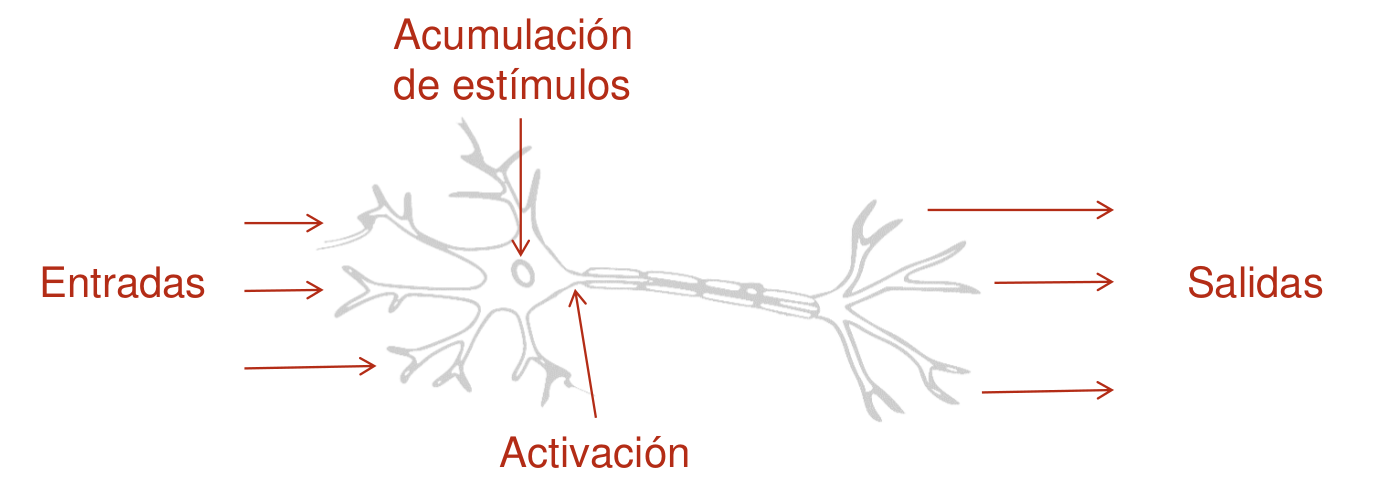
\includegraphics[width=\textwidth]{images/neurona_biologica}
  \caption[Neurona biológica]{Ilustración de una neurona biológica, indicando las equivalencias con la neurona artificial}
  \label{fig:neuron}
\end{figure}

\begin{figure}[hbtp]
  \centering
  
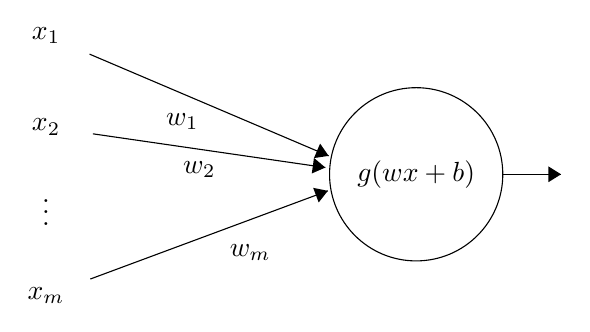
\begin{tikzpicture}[scale=0.2]
\tikzstyle{every node}+=[inner sep=0pt]
\draw [black] (39.4,-29) circle (5.5);
\draw (39.4,-29) node {$g(\Tr wx+b)$};
%\draw (51.6,-29) node {$f$};
\draw [black] (44.9,-29) -- (48.6,-29);
\fill [black] (48.6,-29) -- (47.8,-28.5) -- (47.8,-29.5);

\draw (15.9,-20.2) node {$x_1$};
\draw (15.9,-36.7) node {$x_m$};
\draw (15.9,-30.9) node {$\vdots$};
\draw (15.9,-26) node {$x_2$};
\draw [black] (18.66,-21.37) -- (33.84,-27.83);
\fill [black] (33.84,-27.83) -- (33.3,-27.05) -- (32.91,-27.97);
\draw (24.55,-25.12) node [below] {$w_1$};
\draw [black] (18.87,-26.43) -- (33.63,-28.57);
\fill [black] (33.63,-28.57) -- (32.91,-27.96) -- (32.77,-28.95);
\draw (25.63,-28.16) node [below] {$w_2$};
\draw [black] (18.71,-35.65) -- (33.79,-30.05);
\fill [black] (33.79,-30.05) -- (32.86,-29.86) -- (33.21,-30.79);
\draw (28.87,-33.42) node [below] {$w_m$};
\end{tikzpicture}

  \caption[Neurona artificial]{Una neurona artificial con $m$ entradas y función de activación $g$}
  \label{fig:art-neuron}
\end{figure}

La analogía se lleva a la neurona artificial, como se muestra en la \autoref{fig:art-neuron}, mediante una función de \(\RR^{m}\) en \(\RR\),
donde \(m\) es el número de unidades en la capa anterior. El
comportamiento es similar a una neurona en el sentido de que recoge
información de varias unidades cercanas y calcula su propio valor de
activación, así como la estructuración en capas se ha tomado de la
neurociencia. En la figura \ref{fig:dfnn} se muestra una representación
común de una red neuronal como unidades conectadas formando un grafo.
Las flechas indican el sentido en el que viajan los datos, es decir, las
salidas de funciones que se toman como entradas de otras funciones.

\begin{figure}[hbtp]
  \centering
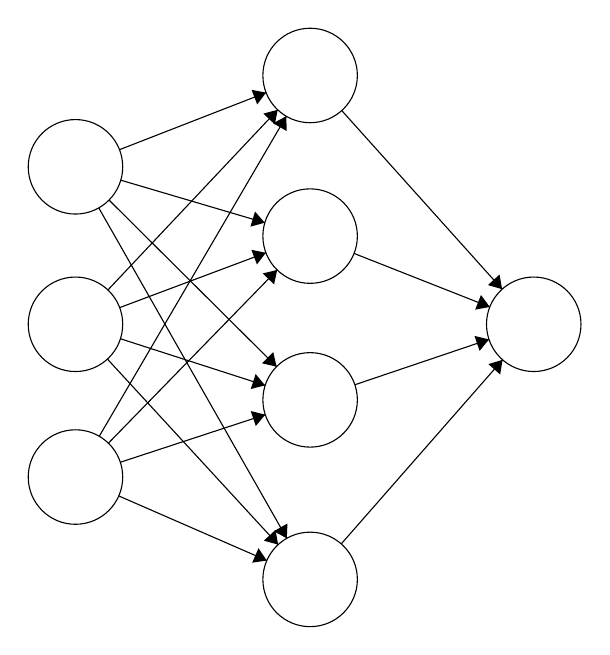
\begin{tikzpicture}[scale=0.2]
\tikzstyle{every node}+=[inner sep=0pt]
\draw [black] (21.5,-13.4) circle (3);
\draw [black] (21.5,-23.4) circle (3);
\draw [black] (21.5,-33.1) circle (3);
\draw [black] (36.4,-7.6) circle (3);
\draw [black] (36.4,-17.8) circle (3);
\draw [black] (36.4,-28.2) circle (3);
\draw [black] (36.4,-39.6) circle (3);
\draw [black] (50.6,-23.4) circle (3);
\draw [black] (24.35,-32.16) -- (33.55,-29.14);
\fill [black] (33.55,-29.14) -- (32.63,-28.91) -- (32.95,-29.86);
\draw [black] (24.25,-34.3) -- (33.65,-38.4);
\fill [black] (33.65,-38.4) -- (33.12,-37.62) -- (32.72,-38.54);
\draw [black] (23.59,-30.95) -- (34.31,-19.95);
\fill [black] (34.31,-19.95) -- (33.39,-20.17) -- (34.11,-20.87);
\draw [black] (23.01,-30.51) -- (34.89,-10.19);
\fill [black] (34.89,-10.19) -- (34.05,-10.63) -- (34.91,-11.13);
\draw [black] (23.56,-21.22) -- (34.34,-9.78);
\fill [black] (34.34,-9.78) -- (33.43,-10.02) -- (34.16,-10.71);
\draw [black] (24.31,-22.34) -- (33.59,-18.86);
\fill [black] (33.59,-18.86) -- (32.67,-18.67) -- (33.02,-19.6);
\draw [black] (24.36,-24.32) -- (33.54,-27.28);
\fill [black] (33.54,-27.28) -- (32.94,-26.56) -- (32.63,-27.51);
\draw [black] (23.53,-25.61) -- (34.37,-37.39);
\fill [black] (34.37,-37.39) -- (34.2,-36.46) -- (33.46,-37.14);
\draw [black] (24.3,-12.31) -- (33.6,-8.69);
\fill [black] (33.6,-8.69) -- (32.68,-8.51) -- (33.04,-9.44);
\draw [black] (24.38,-14.25) -- (33.52,-16.95);
\fill [black] (33.52,-16.95) -- (32.9,-16.24) -- (32.61,-17.2);
\draw [black] (23.63,-15.51) -- (34.27,-26.09);
\fill [black] (34.27,-26.09) -- (34.06,-25.17) -- (33.35,-25.88);
\draw [black] (22.98,-16.01) -- (34.92,-36.99);
\fill [black] (34.92,-36.99) -- (34.96,-36.05) -- (34.09,-36.54);
\draw [black] (38.41,-9.83) -- (48.59,-21.17);
\fill [black] (48.59,-21.17) -- (48.43,-20.24) -- (47.69,-20.91);
\draw [black] (39.19,-18.9) -- (47.81,-22.3);
\fill [black] (47.81,-22.3) -- (47.25,-21.54) -- (46.88,-22.47);
\draw [black] (39.24,-27.24) -- (47.76,-24.36);
\fill [black] (47.76,-24.36) -- (46.84,-24.14) -- (47.16,-25.09);
\draw [black] (38.38,-37.34) -- (48.62,-25.66);
\fill [black] (48.62,-25.66) -- (47.72,-25.93) -- (48.47,-26.59);
\end{tikzpicture}
\caption{\label{fig:dfnn}Ilustración ejemplificando una red neuronal prealimentada de tres capas}
\end{figure}

Para entender cómo las redes prealimentadas aproximan funciones,
consideremos algunos modelos lineales como la regresión lineal o la
logística. Estos modelos tienen claras ventajas, son sencillos, se
pueden ajustar de forma eficiente y fiable. Sin embargo, están muy
limitados, dado que sólo tiene sentido aplicarlos a funciones lineales,
por lo que no pueden sintetizar interacciones entre dos variables de
entrada.

Cuando el objetivo es aproximar funciones no lineales, una vía es
aplicar un modelo lineal no a la variable independiente sino a una
transformación no lineal de la misma. El problema se traduce entonces en
qué transformación \(\phi\) de la variable aplicar para que el modelo
lineal tenga un buen ajuste. Frente a buscar \(\phi\) manualmente, que
requiere extenso conocimiento de cada problema, o usar un \(\phi\) de
muy alta dimensionalidad con capacidad para todos los ejemplos del
conjunto de datos, las redes neuronales realizan un aprendizaje de
\(\phi\) entre una clase de funciones parametrizada: se define un modelo
del tipo

\begin{equation}
  f^{*}(x)\approx f(x;\theta,w)=\Tr{\phi(x;\theta)}w, 
\end{equation}
donde \(\theta\) es un vector de parámetros que facilita escoger una
función \(f\) concreta de entre la clase que define, y \(w\) es otro
vector de parámetros que permite aplicar la transformación obtenida en
la salida deseada. Para encontrar los parámetros que corresponden a una
buena aproximación, se utilizará un algoritmo de optimización basado en
la técnica de gradiente descendente presentada en la sección
\ref{sec:grad-desc}. Se trata de un enfoque muy flexible, ya que se
puede proveer al algoritmo de una clase de funciones más general o más
concreta, según el conocimiento sobre el problema que se posea.

La clase de funciones, dentro de la cual una red neuronal busca la
aproximación, se determina escogiendo la estructura de la red y los
tipos de unidades ocultas y de salida.

\subsection{Funciones de coste}\label{sec:funciones-de-coste}

La mayoría de diseños de redes neuronales involucran definir una
distribución \(P(y\mid x;\theta)\) y aplicar el principio de máxima
verosimilitud. En otros casos, mediante funciones de coste específicas,
se puede predecir simplemente algún estadístico de \(y\) condicionado a
\(x\), en lugar de determinar una distribución de probabilidad.

En el caso más habitual, la función de coste se definirá como la
entropía cruzada (equivalentemente, la log-verosimilitud negativa) entre
la distribución de los datos, \(\hat p\), y la del modelo, \(p\), y
sobre la variable de la salida generada \(y\) respecto de la entrada
\(x\):
\[J(\theta)=C(\hat p(y\mid x), p(y\mid x))=-\E_{\hat p}[\log p(y\mid x)].\]
Una ventaja de este enfoque es que esta función de coste viene determinada
automáticamente por el modelo \(p(y\mid x)\) que escojamos y evita tener
que definir una nueva función para cada modelo. Además, la entropía
cruzada suele permitir calcular gradientes relativamente ``grandes'', en
el sentido de que no se acercan rápidamente a cero, lo cual beneficia al
proceso de optimización.

En ocasiones se añade a la función de coste un término de regularización
o \emph{decaimiento de pesos} de forma que el coste total queda:
\[J(\theta)=C(\hat p, p;y\mid x) + \lambda \Omega(\theta)\]

\subsection{Unidades de salida}\label{unidades-de-salida}

La expresión concreta de la función de coste, cuando la tomamos como la
entropía cruzada, vendrá determinada por la representación de la salida
de la red prealimentada. Estudiamos a continuación el tipo de unidades
que se suelen utilizar para dar dicha salida. Durante el resto de esta
sección, supondremos que la red proporciona un vector de características
\(h=f(x;\theta)\) generado por las unidades ocultas. El cometido de las
unidades de salida es dar una transformación que aporte una salida
apropiada.

\subsubsection{Unidades lineales}\label{unidades-lineales}

Una capa de unidades de este tipo realiza una transformación afín de los
datos: \(\hat y=\Tr Wh+b\). Se suelen utilizar para calcular la media de
una distribución condicional normal: \[p(y\mid x)=\PN(y;\hat t,I).\] En
ese caso, maximizar la entropía cruzada es equivalente a minimizar el
error cuadrático medio.

\subsubsection{Unidades con activación
sigmoidal}\label{unidades-con-activaciuxf3n-sigmoidal}
En muchas tareas, la variable objetivo \(y\) es de tipo binario. Por
ejemplo, los problemas de clasificación binaria son un caso particular
de esta situación. La técnica de máxima verosimilitud lleva a definir
una distribución de Bernoulli sobre \(y\) condicionada a \(x\). Esta
distribución está determinada por un único número en el intervalo
\([0, 1]\), que se corresponde con \(P(y=1\mid x)\).

Para que la unidad de salida tenga un buen comportamiento, es necesario
que no genere gradiente $0$ ni muy cercano a $0$ en casos en los que el
modelo no se acerque a una solución. Esto se consigue utilizando una
\emph{función de activación}, es decir, se compone el cómputo de la
unidad con otra función que la regulariza de alguna manera. En este
caso, se utiliza la función logística:
\[z=\Tr wh+b;\ \hat y = \sigma(z) = \frac{1}{1+e^{-z}}\]

En la \autoref{fig:sigm} se observan los valores en los que se aplica $\sigma$ según el valor de $z$.

\begin{figure}[hbtp]
  \centering
  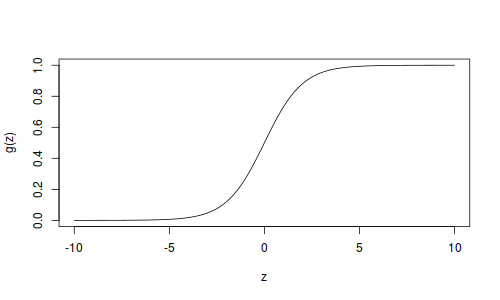
\includegraphics[width=0.7\textwidth]{images/sigmoid.png}
  \caption[Logística]{Gráfica de la función logística}
  \label{fig:sigm}
\end{figure}

Definamos ahora una distribución de probabilidad sobre \(y\), usando el
valor \(z\). Podemos comenzar asumiendo que la probabilidad no
normalizada \(\tilde P\) es log-lineal en \(z\) e \(y\):
\[\log \tilde P(y)=yz,\] y exponenciamos \[\tilde P(y)=e^{yz},\] para
ahora normalizar sobre los valores de \(\tilde P\), obteniendo una
probabilidad \[P(y)=\frac{e^{yz}}{e^{0z}+e^{1z}}=\frac{e^{yz}}{1+e^z}\]
y utilizando de nuevo que \(y\in\{0,1\}\) se tiene

\begin{equation}\label{eq:sigm-prob}
  P(y)=\frac{e^{yz}}{e^{(1-y)z}+e^{yz}}=\frac{1}{\frac{e^{z}}{e^{2yz}}+1}=\sigma((2y-1)z).
\end{equation}

El resultado es una distribución de Bernoulli determinada por una
transformación logística de \(z\). De hecho, puesto que los posibles
valores de \(y\) son $0$ y $1$, también podemos expresarla más claramente
como:
\[P(y)=\sigma(z)^y\sigma(-z)^{1-y}=p^y(1-p)^{1-y}\mbox{ donde }p=\sigma(z).\]

Ahora, la función de coste para esta distribución, tomando la entropía
cruzada y usando \eqref{eq:sigm-prob}, es:
\[J(\theta)=-\log P(y\mid x)=-\log\sigma((2y-1)z).\]

Dado que la función logística está valuada en el intervalo abierto
\(]0,1[\), su logaritmo es finito y \(J\) está bien definida.

\subsubsection{\texorpdfstring{Unidades con activación
\emph{softmax}}{Unidades con activación softmax}}\label{unidades-con-activaciuxf3n-softmax}

Las unidades con función de activación \emph{softmax} se emplean cuando
se pretende representar una distribución de probabilidad sobre una
variable discreta con un número finito de valores. Generalmente, esta
situación se da en problemas de clasificación multiclase. Así, se pueden
interpretar como una generalización de las unidades sigmoidales.

Mientras que para caracterizar una variable binaria bastaba con una sola
unidad de salida (la salida era un escalar entre $0$ y $1$), ahora se
utilizarán tantas unidades como posibles valores puedar tomar la variable. Si
\(y\) puede tomar uno de entre \(n\) posibles valores, la capa de salida
con \emph{softmax} generará un vector \(\hat y\) donde
\(\hat y_i=P(y=i\mid x)\), exigiendo que \(\sum_{i=1}^n\hat y_i=1\).

La función vectorial \emph{softmax} se define en cada componente
\(i=1,\dots,n\) como

\begin{equation}\label{eq:softmax}
  \softmax{z}_i = \frac{\exp(z_i)}{\sum_{j=1}^{n}\exp(z_j)}.
\end{equation}

El vector \(z\) al que se aplica la función se obtiene de una capa de
unidades lineales que proporcionan probabilidades logarítmicas sin
normalizar:
\[z=\Tr Wh+b;\ z_{i}=\log\tilde P(y=i\mid x).\]

De nuevo, la
función de coste se puede definir siguiendo la misma técnica, mediante
la entropía cruzada.

\subsection{Unidades ocultas}\label{unidades-ocultas}

Cualquiera de los tipos anteriores de unidad se puede utilizar en una
capa oculta, pero existen más y el diseño de unidades ocultas es un
campo de investigación muy activo, pese a la falta de principios
teóricos que lo guíen. A continuación se exponen algunos de los tipos
más usuales. Salvo que se indique lo contrario, todas las capas de
unidades calculan una transformación afín \[z= \Tr Wx+b,\] donde \(x\) es
el vector de entrada, equivalentemente, el vector de salida de la capa
inmediatamente anterior o un vector de datos si se trata de la primera
capa. Se compone esta transformación con la función de activación
específica a cada tipo de unidad.

\subsubsection{Unidades lineales rectificadas
(ReLU)}\label{unidades-lineales-rectificadas-relu}

La función de activación de las unidades lineales rectificadas
(\emph{Rectified Linear Units}, ReLU) es

\begin{equation}
g(z)_i=\max\{0,z_i\}.
\end{equation}

Se muestra en la \autoref{fig:relu} el valor que toma la ReLU según el valor de $z_i$.

\begin{figure}[hbtp]
  \centering
  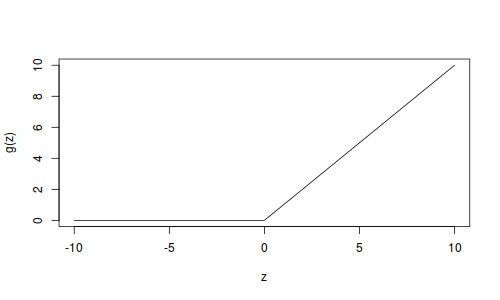
\includegraphics[width=0.7\textwidth]{images/relu.png}
  \caption[ReLU]{Gráfica de la función de activación de una ReLU}
  \label{fig:relu}
\end{figure}

Estas unidades son fáciles de optimizar ya que son similares a las
unidades lineales. Aunque no es diferenciable en \(z=0\), se pueden
utilizar algoritmos basados en gradiente para optimizar la función
objetivo. Esto es debido a que, generalmente, durante el entrenamiento
no se llega a un punto en el que el gradiente sea exactamente $0$, así que
se pueden aceptar puntos donde el gradiente no esté definido en los
mínimos de la función coste.

\subsubsection{Extensiones de ReLU}\label{extensiones-de-relu}

Algunas generalizaciones de las ReLU modifican el gradiente cuando las
componentes de \(z\) son negativas:

\begin{itemize}
\tightlist
\item
  \textbf{Rectificación por valor absoluto}:
  \(g(z)_{i}=\lvert z_{i} \rvert\)
\item
  \textbf{\emph{Leaky} ReLU}: \(g(z)_i=\max(0,z_i)+\alpha\min(0,z_i)\)
  con \(\alpha\) pequeño como \(0,01\) (\autoref{fig:leaky})
\item
  \textbf{ReLU paramétrica}: \(g(z)_i=\max(0,z_i)+\alpha_i\min(0,z_i)\),
  con \(\alpha_i\) como un parámetro optimizable
\end{itemize}

\begin{figure}[hbtp]
  \centering
  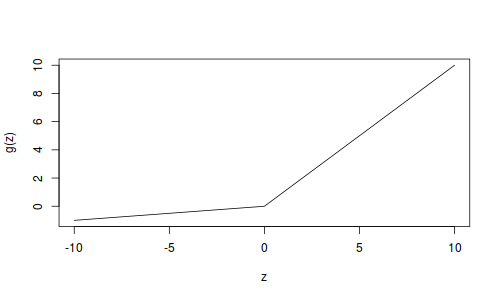
\includegraphics[width=0.7\textwidth]{images/leaky.png}
  \caption[Leaky ReLU]{Función de activación de una \emph{leaky} ReLU para $\alpha=0.1$}
  \label{fig:leaky}
\end{figure}

Las capas de \textbf{unidades \emph{maxout}} agrupan las componentes de
\(z\) en conjuntos de \(k\) valores cada uno. Cada una de las unidades
de la capa proporciona entonces el máximo de uno de esos conjuntos:
\[g(z)_i=\max\{z_j:j\in S_i\},\ S_i=\{(i-1)k + 1, (i-1)k + 2,\dots, ik\}.\]
En este caso, si \(z\in\RR^{kd}\), entonces \(g(z)\in\RR^{d}\). El
aspecto interesante de las unidades \emph{maxout} es el hecho de que una
capa de ellas puede aprender una función convexa lineal a trozos de
hasta \(k\) trozos. Podemos intuir que una capa de este tipo podrá
aproximar cualquier función convexa con precisión arbitraria para un
\(k\) conveniente.

\subsubsection{Unidades con activación sigmoidal o tangente
hiperbólica}\label{unidades-con-activaciuxf3n-sigmoidal-o-tangente-hiperbuxf3lica}

Otras dos funciones muy comunes para la activación de unidades en redes
neuronales son la función logística

\begin{equation}
  g(z)_i=\sigma(z_i)=\frac{1}{1+e^{-z_i}},
\end{equation}
y la tangente hiperbólica (\autoref{fig:tanh})
\begin{equation}
  g(z)_i=\tanh(z_i)=\frac{e^{z_i}-e^{-z_i}}{e^{z_i}+e^{-z_i}}.
\end{equation}

\begin{figure}[hbtp]
  \centering
  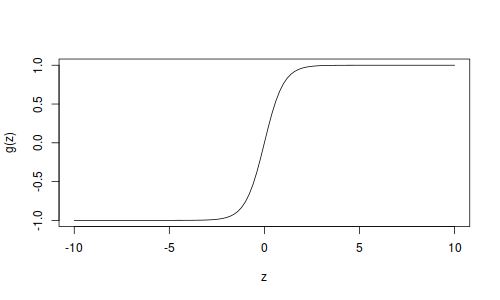
\includegraphics[width=0.7\textwidth]{images/tanh.png}
  \caption[$\tanh$]{Gráfica de la función tangente hiperbólica}
  \label{fig:tanh}
\end{figure}

Se puede comprobar que \(\tanh(z_i)=2\sigma(2z_i)-1\).

El uso de estas unidades era más común antes de la aparición de las
ReLU. En la actualidad está decreciendo su uso.

\subsubsection{Otras unidades ocultas}\label{otras-unidades-ocultas}

Para construir otros tipos de unidad oculta simplemente basta con elegir
otra función de activación. Las siguientes son algunas relativamente
comunes:

\begin{itemize}
\tightlist
\item
  El \textbf{coseno} \(g(z)_i=cos(z_i)\) ha sido usada por
  \textcite{goodfellow2016} en el conocido conjunto MNIST obteniendo una
  tasa de error inferior al 1\%.
\item
  La \textbf{identidad} \(g(z) = z\) se puede utilizar para encadenar
  capas de forma lineal y utilizar alguna función de activación
  diferente a la salida.
\item
  La función \emph{softplus} \(g(z)_i=\zeta(z_i)=\log(1+e^{z_i})\) es
  una versión infinitamente derivable de la unidad lineal rectificada (\autoref{fig:softplus}).
  Sin embargo, en la práctica no suele presentar ventajas sobre la ReLU.
\end{itemize}

\begin{figure}[hbtp]
  \centering
  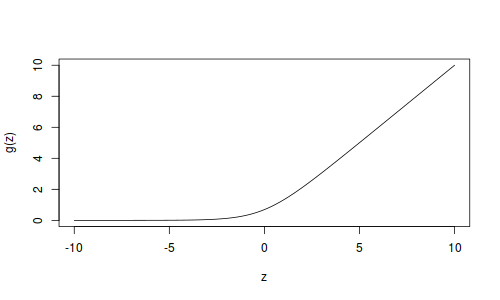
\includegraphics[width=0.7\textwidth]{images/softplus.png}
  \caption[Softplus]{Gráfica de la función \emph{softplus}}
  \label{fig:softplus}
\end{figure}

\section{Entrenamiento de redes neuronales
profundas}\label{entrenamiento-de-redes-neuronales-profundas}

El proceso de entrenamiento de una red neuronal profunda
requiere realizar observaciones sobre las salidas a partir de los datos
de entrada, y evaluar el error cometido respecto a las salidas deseadas.
Para calcular la salida de la red $f(x)$ frente a una instancia $x$ se
utiliza el mecanismo de propagación hacia adelante, en el que intuitivamente
podemos decir que los datos ``atraviesan'' la red. La evaluación de la
red se realiza en base a una función de coste y posteriormente se deben
actualizar los parámetros para alterar la función $f$, para lo cual es
necesario calcular el gradiente de dicho coste. El cómputo del gradiente
se obtiene mediante la técnica de propagación hacia atrás.

\subsection{Propagación hacia
adelante}\label{propagaciuxf3n-hacia-adelante}

Las redes neuronales prealimentadas, que se han estudiado en la sección
\ref{sec:feedforward}, son funciones que aceptan vectores de entrada y
procesan la información computando varias funciones intermedias,
propagando así la información, hasta la salida de la red. Este proceso
se denomina \emph{propagación hacia adelante}, y se describe en el
algoritmo \ref{alg:fwdprop}.

\begin{algorithm}
\caption{Propagación hacia adelante en una red neuronal profunda con función de activación $g$, y cálculo de la función de coste $J$, para una instancia $x$ (en la práctica se utilizan minilotes de instancias)}
\label{alg:fwdprop}
\begin{algorithmic}
  \REQUIRE{profundidad de la red $l$}
  \REQUIRE{$W^{(i)}$ matriz de pesos de la capa $i$-ésima}
  \REQUIRE{$b^{(i)}$ vector de sesgos de la capa $i$-ésima}
  \REQUIRE{instancia $x$ a procesar}
  \REQUIRE{salida objetivo $y^{*}$}
  \STATE{$h^{(0)}\gets x$}
  \FOR{$k=1,\dots,l$}
  \STATE{$z^{(k)}\gets W^{(k)}h^{(k-1)}+b^{(k)}$}
  \STATE{$h^{(k)}\gets g(z^{(k)})$}
  \ENDFOR
  \STATE{$y\gets h^{(l)}$}
  \STATE{Se calcula la función de coste mediante una distancia o pérdida entre la salida obtenida y la deseada, y un término de regularización $\Omega$:}
  \STATE{$J\gets L(y,y^{*})+\lambda \Omega(\theta)$}
\end{algorithmic}
\end{algorithm}

\subsection{Propagación hacia
atrás}\label{sec:backprop}

Consideremos una red neuronal prealimentada profunda, determinada por un
vector de parámetros \(\theta\). Durante el entrenamiento, la salida
generada por la propagación hacia adelante se compara con la salida
deseada y se calcula un coste \(J(y,y^{*};\theta)\in\RR\). Para aplicar
un algoritmo de optimización basado en gradiente descendente (se
estudiarán en la sección \ref{sec:dl-opt}), es necesario conocer el
gradiente de la función \(J\) respecto de los parámetros \(\theta\).
Este gradiente se puede calcular analíticamente, pero evaluar
\(\nabla_{\theta} J(y,y^{*};\theta)\) es generalmente muy costoso
computacionalmente. El algoritmo de propagación hacia atrás, o
\emph{backprop}, realiza este cálculo de forma eficiente.

\begin{example}
  
Consideremos la red neuronal de la figura \ref{fig:ex-backprop}. Suponiendo que cada neurona utiliza la misma función de activación $g$, podemos dar una expresión de $f$ acorde con los pesos y sesgos que se muestran en la imagen.

  \begin{figure}[hbtp]
\centering
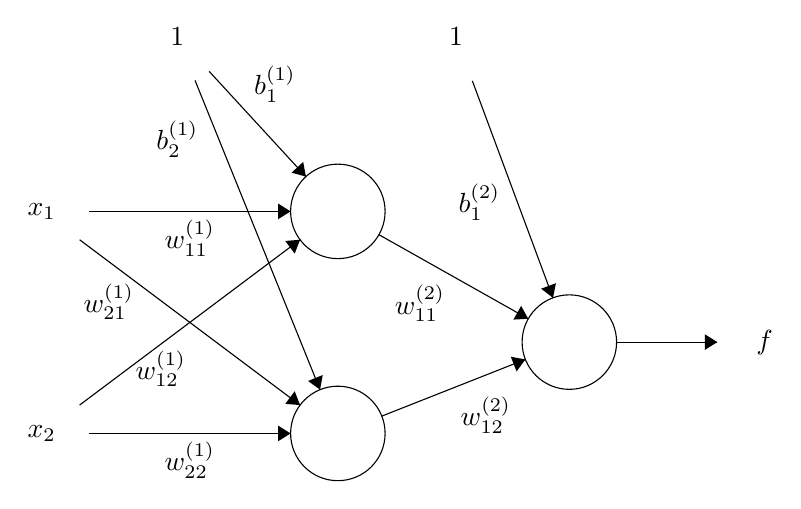
\begin{tikzpicture}[scale=0.2]
\tikzstyle{every node}+=[inner sep=0pt]
\draw [black] (34,-24.7) circle (3);
\draw [black] (34,-38.8) circle (3);
\draw [black] (48.7,-33) circle (3);
\draw (15.2,-24.7) node {$x_1$};
\draw (15.2,-38.8) node {$x_2$};
\draw (61.1,-33) node {$f$};
\draw (23.8,-13.6) node {$1$};
\draw (41.5,-13.6) node {$1$};
\draw [black] (36.79,-37.7) -- (45.91,-34.1);
\fill [black] (45.91,-34.1) -- (44.98,-33.93) -- (45.35,-34.86);
\draw (43.4,-36.44) node [below] {$w_{12}^{(2)}$};
\draw [black] (36.61,-26.18) -- (46.09,-31.52);
\fill [black] (46.09,-31.52) -- (45.64,-30.7) -- (45.15,-31.57);
\draw (39.21,-29.35) node [below] {$w_{11}^{(2)}$};
\draw [black] (17.6,-26.5) -- (31.6,-37);
\fill [black] (31.6,-37) -- (31.26,-36.12) -- (30.66,-36.92);
\draw (19.45,-29.25) node [below] {$w_{21}^{(1)}$};
\draw [black] (17.6,-37) -- (31.6,-26.5);
\fill [black] (31.6,-26.5) -- (30.66,-26.58) -- (31.26,-27.38);
\draw (22.75,-33.50) node [below] {$w_{12}^{(1)}$};
\draw [black] (51.7,-33) -- (58.1,-33);
\fill [black] (58.1,-33) -- (57.3,-32.5) -- (57.3,-33.5);
\draw [black] (25.83,-15.81) -- (31.97,-22.49);
\fill [black] (31.97,-22.49) -- (31.8,-21.56) -- (31.06,-22.24);
\draw (31.36,-16.61) node [left] {$b_1^{(1)}$};
\draw [black] (42.54,-16.41) -- (47.66,-30.19);
\fill [black] (47.66,-30.19) -- (47.85,-29.26) -- (46.91,-29.61);
\draw (44.34,-24.11) node [left] {$b_1^{(2)}$};
\draw [black] (24.93,-16.38) -- (32.87,-36.02);
\fill [black] (32.87,-36.02) -- (33.04,-35.09) -- (32.11,-35.47);
\draw (25.16,-20.1) node [left] {$b_2^{(1)}$};
\draw [black] (18.2,-24.7) -- (31,-24.7);
\fill [black] (31,-24.7) -- (30.2,-24.2) -- (30.2,-25.2);
\draw (24.6,-25.2) node [below] {$w_{11}^{(1)}$};
\draw [black] (18.2,-38.8) -- (31,-38.8);
\fill [black] (31,-38.8) -- (30.2,-38.3) -- (30.2,-39.3);
\draw (24.6,-39.3) node [below] {$w_{22}^{(1)}$};
\end{tikzpicture}
\caption{\label{fig:ex-backprop}Red neuronal sencilla de dos capas con entrada vectorial de dos componentes, se marcan los pesos y los sesgos en cada conexión}
\end{figure}

En este caso, el vector de parámetros que determina la red será
$$\theta=\left(w_{11}^{(1)},w_{12}^{(1)},w_{21}^{(1)},w_{22}^{(1)},b_{1}^{(1)},b_{2}^{(1)},w_{11}^{(2)},w_{12}^{(2)},b_{1}^{(2)}\right).$$
Puesto que la función de coste $J$ vendrá determinada por el valor de $f$ en el mismo punto, para calcular su gradiente nos interesa conocer el de $f$. La expresión desarrollada de $f$ queda\footnotesize
\begin{gather*}
f(x_1,x_2;\theta)=\\g\left(w_{11}^{(2)}g\left(w_{11}^{(1)}x_{1}+w_{12}^{(1)}x_2+b_1^{(1)}\right)+w_{12}^{(2)}g\left(w_{21}^{(1)}x_1+w_{22}^{(1)}x_2+b_2^{(1)}\right)+b_1^{(2)}\right).
\end{gather*}\normalsize

Ahora, mediante la regla de la cadena podemos desarrollar la parcial de $f$ respecto de cualquiera de los parámetros. Llamamos
\footnotesize
\begin{align*}
  \alpha&=g'\left(w_{11}^{(2)} g\left(w_{11}^{(1)}x_{1}+w_{12}^{(1)}x_2+b_1^{(1)}\right) + w_{12}^{(2)} g\left(w_{21}^{(1)}x_1+w_{22}^{(1)}x_2+b_2^{(1)}\right)+b_1^{(2)}\right)\\
  \beta&=g'\left(w_{11}^{(1)}x_{1}+w_{12}^{(1)}x_2+b_1^{(1)}\right)\\
  \gamma&=g'\left(w_{21}^{(1)}x_{1}+w_{22}^{(1)}x_2+b_2^{(1)}\right)
\end{align*}
\normalsize
y se tiene
\footnotesize
\begin{alignat*}{3}
  \frac{\partial f}{\partial w_{11}^{(1)}}(x_1,x_2;\theta)&=\alpha w_{11}^{(2)}\beta x_1,\quad&
  \frac{\partial f}{\partial w_{12}^{(1)}}(x_1,x_2;\theta)&=\alpha w_{11}^{(2)}\beta x_2,\\
  \frac{\partial f}{\partial w_{21}^{(1)}}(x_1,x_2;\theta)&=\alpha w_{12}^{(2)}\gamma x_1,\quad&
  \frac{\partial f}{\partial w_{22}^{(1)}}(x_1,x_2;\theta)&=\alpha w_{12}^{(2)}\gamma x_2,\\
  \frac{\partial f}{\partial b_{1}^{(1)}}(x_1,x_2;\theta)&=\alpha w_{11}^{(2)}\beta, \quad&
  \frac{\partial f}{\partial b_{2}^{(1)}}(x_1,x_2;\theta)&=\alpha w_{12}^{(2)}\gamma, \\
  \frac{\partial f}{\partial w_{11}^{(2)}}(x_1,x_2;\theta)&=\alpha g(w_{11}^{(1)}x_{1}+w_{12}^{(1)}x_2 + b_1^{(1)}),&&\\
  \frac{\partial f}{\partial w_{12}^{(2)}}(x_1,x_2;\theta)&=\alpha g(w_{21}^{(1)}x_{1}+w_{22}^{(1)}x_2 + b_2^{(1)}),&\quad
  \frac{\partial f}{\partial b_{1}^{(2)}}(x_1,x_2;\theta)&=\alpha.
\end{alignat*}
\normalsize

Como podemos observar, algunos de los factores de las parciales se repiten en varias de ellas, de forma que se ahorrarán muchos cálculos innecesarios si no se repiten. Este hecho se hace aún más evidente conforme se añaden capas a la red y unidades a cada capa. Por ello, el algoritmo de propagación hacia atrás permite optimizar el cálculo del gradiente mediante varios pasos intermedios para evitar cálculos repetidos.

\end{example}

En el algoritmo \ref{alg:backprop} se describe \emph{backprop} paso a
paso. Es fácil comprobar que aplicando esta técnica al ejemplo anterior
podemos evaluar las parciales que se han deducido sin repetir cálculos
costosos.

\begin{algorithm}
\caption{Propagación hacia atrás}
\label{alg:backprop}
\begin{algorithmic}
\STATE{Tras la propagación hacia adelante, calcular el gradiente de la capa de salida:}
\STATE{$d\gets \nabla_{y}J(y,y^{*};\theta)=\nabla_{y}L(y,y^{*})$}
  \FOR{$k=l,\dots,1$}
  \STATE{Aplicar la regla de la cadena a la función de activación ($\odot$ denota producto componente a componente):}
  \STATE{$d\gets \nabla_{z^{(k)}}J=d\odot g'(z^{i})$}
  \STATE{Calcular gradientes en los pesos y sesgos (incluyendo el término de regularización si es necesario):}
  \STATE{$\nabla_{b^{(k)}}J=d+\lambda\nabla_{b^{(k)}}\Omega(\theta)$}
  \STATE{$\nabla_{W^{(k)}}J=d\Tr{(h^{(k-1)})}+\lambda\nabla_{W^{(k)}}\Omega(\theta)$}
  \STATE{Propagar el gradiente hacia la capa oculta anterior:}
  \STATE{$d\gets \nabla_{h^{(k-1)}}J=\Tr{(W^{(k)})}d$}
  \ENDFOR
\end{algorithmic}
\end{algorithm}

\section{Optimización en Deep
Learning}
\label{sec:dl-opt}

Como se ha visto, una red profunda define una función $f$ que queda
determinada por una secuencia finita de parámetros. Estos parámetros se deben
optimizar para que la salida de la red sea lo más próxima posible a la
salida deseada. Para ello, sería interesante utilizar la técnica de
gradiente descendente estudiada en la \autoref{sec:grad-desc}. Sin embargo,
el coste computacional de calcular el gradiente respecto del conjunto
de datos al completo lo hace inviable. En esta sección se introducen
algoritmos derivados de gradiente descendente que aproximan el mismo
comportamiento pero resultan mucho más eficientes.

\subsection{Gradiente descendente estocástico
(SGD)}\label{gradiente-descendente-estocuxe1stico-sgd}\label{sec:sgd}

En aprendizaje automático, y especialmente en Deep Learning, es común
utilizar conjuntos de datos con un gran número de instancias, para
favorecer la capacidad de generalización de los modelos producidos por
los algoritmos. Esto provoca que el coste computacional de calcular cada
paso de un gradiente descendente haga inviable su uso. Sin embargo, se
puede utilizar una aproximación estocástica al algoritmo denominada
gradiente descendente estocástico (\emph{Stochastic Gradient Descent},
SGD). En esta versión de gradiente descendente se asienta la mayor
parte del desarrollo del Deep Learning en la actualidad.

Al ser una aproximación estocástica, SGD calcula un estimador del
gradiente de la función objetivo a partir de un número reducido de
muestras. Se describe en el algoritmo \ref{alg:sgd}.

\begin{algorithm}
\caption{Gradiente descendente estocástico, iteración $k$-ésima}
\label{alg:sgd}
\begin{algorithmic}
  \REQUIRE{Tasa de aprendizaje $\varepsilon_k$}
  \REQUIRE{Parámetro inicial $\theta$}
  \WHILE{no se alcanza criterio de parada}
  \STATE{Escoger un minilote de $m$ instancias del conjunto de entrenamiento $x^{(1)},\dots,x^{(m)}$ con correspondientes objetivos $y^{(i)}$}
  \STATE{Calcular estimador del gradiente: $\hat g\gets \frac 1 m \nabla \sum_i L(f(x^{(i)}; \theta),y^{(i)})$}
  \STATE{Actualizar parámetro: $\theta\gets\theta - \varepsilon_k\hat g$}
  \ENDWHILE
\end{algorithmic}
\end{algorithm}

\subsection{Variantes de SGD}\label{variantes-de-sgd}

Existen múltiples variantes de SGD que adaptan el aprendizaje de distintas formas a lo largo de las iteraciones. En muchos casos mejoran respecto al comportamiento de SGD pero esto varía según el conjunto de datos tratado.

\begin{itemize}
\item \textbf{SGD con momento:} el momento es un término adicional que fuerza a que SGD varíe menos la
dirección de una iteración a otra. De esta forma, el zigzagueo
característico de GD, también presente en SGD, se atenúa. Esta versión
se describe en el algoritmo \ref{alg:sgdm}.
\item \textbf{AdaGrad} \autocite{adagrad} es una versión adaptativa de SGD, en el
sentido de que varía los parámetros de forma inversamente proporcional a
la raíz cuadrada de la suma de los cuadrados de los valores anteriores.
Así, en lugar de decrementar la tasa de aprendizaje de igual forma para
todos los parámetros, la decrementa más rápido en los parámetros que
tienen mayores derivadas parciales. Como resultado adicional, en las
zonas de menor pendiente del espacio de parámetros el algoritmo progresa
más rápidamente que SGD. Se describe en el algoritmo \ref{alg:adagrad}.
\item \textbf{RMSProp}, detallado en el algoritmo \ref{alg:rmsprop},
sustituye la acumulación de gradientes de AdaGrad por una media
exponencial, de forma que tenga mejor comportamiento al optimizar
funciones no convexas.
\item \textbf{Adam} es un algoritmo que también adapta la tasa de aprendizaje y además
introduce un momento adaptativo, se puede considerar una combinación de
RMSProp con momento. Se describe en el algoritmo \ref{alg:adam}.

\end{itemize}

\begin{algorithm}
\caption{Gradiente descendente estocástico con momento}
\label{alg:sgdm}
\begin{algorithmic}
  \REQUIRE{Tasa de aprendizaje $\varepsilon$, momento $\alpha$}
  \REQUIRE{Parámetro inicial $\theta$, velocidad inicial $v$}
  \WHILE{no se alcanza criterio de parada}
  \STATE{Escoger un minilote de $m$ instancias del conjunto de entrenamiento $x^{(1)},\dots,x^{(m)}$ con correspondientes objetivos $y^{(i)}$}
  \STATE{Calcular estimador del gradiente: $\hat g\gets \frac 1 m \nabla \sum_i L(f(x^{(i)}; \theta),y^{(i)})$}
  \STATE{Actualizar la velocidad: $v\gets\alpha v - \varepsilon \hat g$}
  \STATE{Actualizar parámetro: $\theta\gets\theta + v$}
  \ENDWHILE
\end{algorithmic}
\end{algorithm}

\begin{algorithm}
\caption{Adagrad}
\label{alg:adagrad}
\small
\textbf{Notación:} $\odot$ es el producto componente a componente, $\sqrt{.}$ es la raíz cuadrada componente a componente y la división por $\frac{1}{\delta + \sqrt r}$ se realiza componente a componente.
\begin{algorithmic}
  \small
  \REQUIRE{Tasa de aprendizaje $\varepsilon$, constante pequeña $\delta$}
  \REQUIRE{Parámetro inicial $\theta$}
  \STATE{Inicializar: $r\gets 0$}
  \WHILE{no se alcanza criterio de parada}
  \STATE{Escoger un minilote de $m$ instancias del conjunto de entrenamiento $x^{(1)},\dots,x^{(m)}$ con correspondientes objetivos $y^{(i)}$}
  \STATE{Calcular estimador del gradiente: $\hat g\gets \frac 1 m \nabla \sum_i L(f(x^{(i)}; \theta),y^{(i)})$}
  \STATE{Acumular cuadrado del gradiente: $r\gets r + \hat g\odot \hat g$}
  \STATE{Calcular actualización: $\Delta\theta\gets - \frac{\varepsilon}{\delta + \sqrt{r}}\odot \hat g$}
  \STATE{Actualizar parámetro: $\theta\gets\theta + \Delta\theta$}
  \ENDWHILE
\end{algorithmic}
\end{algorithm}


\begin{algorithm}
\caption{RMSProp}
\label{alg:rmsprop}
\textbf{Notación:} De nuevo, las operaciones $\odot$, raíz cuadrada y división se realizan componente a componente.
\begin{algorithmic}
  \REQUIRE{Tasa de aprendizaje $\varepsilon$, constante pequeña $\delta$}
  \REQUIRE{Tasa de decaimiento $\rho$}
  \REQUIRE{Parámetro inicial $\theta$}
  \STATE{Inicializar: $r\gets 0$}
  \WHILE{no se alcanza criterio de parada}
  \STATE{Escoger un minilote de $m$ instancias del conjunto de entrenamiento $x^{(1)},\dots,x^{(m)}$ con correspondientes objetivos $y^{(i)}$}
  \STATE{Calcular estimador del gradiente: $\hat g\gets \frac 1 m \nabla \sum_i L(f(x^{(i)}; \theta),y^{(i)})$}
  \STATE{Acumular cuadrado del gradiente: $r\gets \rho r + (1 - \rho) \hat g\odot \hat g$}
  \STATE{Calcular actualización: $\Delta\theta\gets - \frac{\varepsilon}{\sqrt{\delta + r}}\odot \hat g$}
  \STATE{Actualizar parámetro: $\theta\gets\theta + \Delta\theta$}
  \ENDWHILE
\end{algorithmic}
\end{algorithm}

\begin{algorithm}
\caption{Adam}
\label{alg:adam}
\begin{algorithmic}
  \REQUIRE{Tasa de aprendizaje $\varepsilon$, constante pequeña $\delta$}
  \REQUIRE{Tasas de decaimiento exponencial $\rho_{1}, \rho_2\in[0,1[$}
  \REQUIRE{Parámetro inicial $\theta$}
  \STATE{Inicializar: $s\gets 0, r\gets 0, t\gets 0$}
  \WHILE{no se alcanza criterio de parada}
  \STATE{Escoger un minilote de $m$ instancias del conjunto de entrenamiento $x^{(1)},\dots,x^{(m)}$ con correspondientes objetivos $y^{(i)}$}
  \STATE{Calcular estimador del gradiente: $\hat g\gets \frac 1 m \nabla \sum_i L(f(x^{(i)}; \theta),y^{(i)})$}
  \STATE{Incrementar tiempo: $t\gets t + 1$}
  \STATE{Actualizar estimador sesgado del 1er momento: $s\gets \rho_1 s + (1 - \rho_1)\hat g$}
  \STATE{Actualizar estimador sesgado del 2º momento: $r\gets \rho_2 s + (1 - \rho_2)\hat g\odot \hat g$}
  \STATE{Corregir sesgos: $\hat s\gets\frac{s}{1 - \rho_1^t},\ \hat r\gets\frac{r}{1 - \rho_2^t}$}
  \STATE{Calcular actualización: $\Delta\theta\gets - \frac{\varepsilon}{\delta + \sqrt{\hat r}}\hat s$ (operaciones componente a componente)}
  \STATE{Actualizar parámetro: $\theta\gets\theta + \Delta\theta$}
  \ENDWHILE
\end{algorithmic}
\end{algorithm}

\section{Estructuras profundas no
supervisadas}\label{estructuras-profundas-no-supervisadas}

En esta sección nos centramos en las estructuras dedicadas a aprendizaje no supervisado en Deep Learning. Estudiaremos las máquinas de Boltzmann restringidas (\textit{Restricted Boltzmann Machine}, RBM) y los autoencoders y sus variantes. También analizaremos una propuesta de entrenamiento específica para autoencoders. La fuente principal de esta sección es \textcite[capítulos 14 y 20]{goodfellow2016}.

\subsection{Máquina de Boltzmann restringida
(RBM)}\label{muxe1quina-de-boltzmann-restringidas-rbm}

Las máquinas de Boltzmann restringidas o RBMs son modelos basados en energía no direccionales. No son por sí mismas modelos profundos, pero son la base de algunas arquitecturas de Deep Learning como las \textit{Deep Belief Networks} \autocite{hinton2006dbn}. Contienen una capa de variables observables o visibles y una sola capa de variables ocultas o latentes.

Se denominan restringidas porque, a diferencia de las máquinas de Boltzmann generales, forman grafos bipartitos donde no hay conexiones entre unidades de la misma capa, como se puede observar en la \autoref{fig:rbm}. Que sean modelos basados en energía quiere decir que la distribución de probabilidad $\tilde p$ que aprenden viene dada de la forma
\[
  \tilde p(x)=e^{-E(x)}~,
\]
donde la función $E$ se llama \textit{función de energía}. Por último, son no direccionales ya que las conexiones entre unidades funcionan en ambos sentidos.

\begin{figure}[hbtp]
  \centering
  
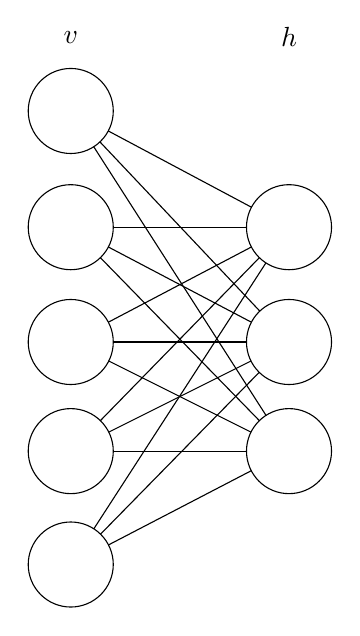
\begin{tikzpicture}[scale=0.18]
\tikzstyle{every node}+=[inner sep=0pt]
\draw [black] (13.9,-15.6) circle (3);
\draw [black] (13.9,-23.8) circle (3);
\draw [black] (13.9,-31.9) circle (3);
\draw [black] (13.9,-39.6) circle (3);
\draw [black] (13.9,-47.6) circle (3);
\draw [black] (29.3,-23.8) circle (3);
\draw [black] (29.3,-31.9) circle (3);
\draw [black] (29.3,-39.6) circle (3);
\draw (13.9,-10.4) node {$v$};
\draw (29.3,-10.4) node {$h$};
\draw [black] (16.55,-17.01) -- (26.65,-22.39);
\draw [black] (15.96,-17.78) -- (27.24,-29.72);
\draw [black] (15.52,-18.12) -- (27.68,-37.08);
\draw [black] (16.9,-23.8) -- (26.3,-23.8);
\draw [black] (16.56,-25.2) -- (26.64,-30.5);
\draw [black] (15.99,-25.95) -- (27.21,-37.45);
\draw [black] (16.56,-30.5) -- (26.64,-25.2);
\draw [black] (16.9,-31.9) -- (26.3,-31.9);
\draw [black] (16.58,-33.24) -- (26.62,-38.26);
\draw [black] (15.99,-37.45) -- (27.21,-25.95);
\draw [black] (16.58,-38.26) -- (26.62,-33.24);
\draw [black] (16.9,-39.6) -- (26.3,-39.6);
\draw [black] (15.53,-45.08) -- (27.67,-26.32);
\draw [black] (16,-45.46) -- (27.2,-34.04);
\draw [black] (16.56,-46.22) -- (26.64,-40.98);
\end{tikzpicture}
  \caption[Máquina de Boltzmann restringida]{Ilustración de las unidades de una máquina de Boltzmann restringida y las conexiones entre ellas}
  \label{fig:rbm}
\end{figure}

Las RBMs en su versión básica sólo contemplan valores binarios en las variables. Formalmente, si $V$ es un vector de variables aleatorias binarias observables, y llamamos $H$ al vector de variables aleatorias binarias ocultas, la distribución conjunta representada por la RBM asociada es
\[
  P(V=v,H=h)=\frac 1 Z e^{-E(v,h)}~,
\]
donde la función de energía $E$ viene dada por la expresión
\[
  E(v,h)=-\Tr b v -\Tr c h - \Tr v W h~,
\]
y $Z$ es la constante de normalización correspondiente:
\[
Z=\sum_{v}\sum_{h}e^{-E(v,h)}~.
\]

Puesto que dicha constante $Z$ es, en general, demasiado costosa de calcular como para que sea factible la evaluación directa de $P(v, h)$, se suelen utilizar otras técnicas para entrenar un modelo de RBM. Estas incluyen \textit{Contrastive Divergence} \autocite{hinton2002cd} y máxima verosimilitud estocástica, conocida también como \textit{Persistent Contrastive Divergence} \autocite{tieleman2008pcd}.

\subsection{Autoencoder}\label{sec:autoencoder}

Un autoencoder es una red neuronal que se entrena con el objetivo de reproducir la entrada a su salida. Internamente, contiene una capa oculta que describe un código utilizado para representar la entrada. Se puede considerar una red compuesta por dos partes: una función codificadora $f$ que transforma la entrada en el código, y una función decodificadora $g$ que se aplica al código y trata de reconstruir la entrada. Una ilustración de la arquitectura se muestra en la \autoref{fig:autoencoder}, donde la etapa de codificación se realiza entre la primera y la segunda capa, y la decodificación entre la segunda y la última.

\begin{figure}[hbtp]
  \centering
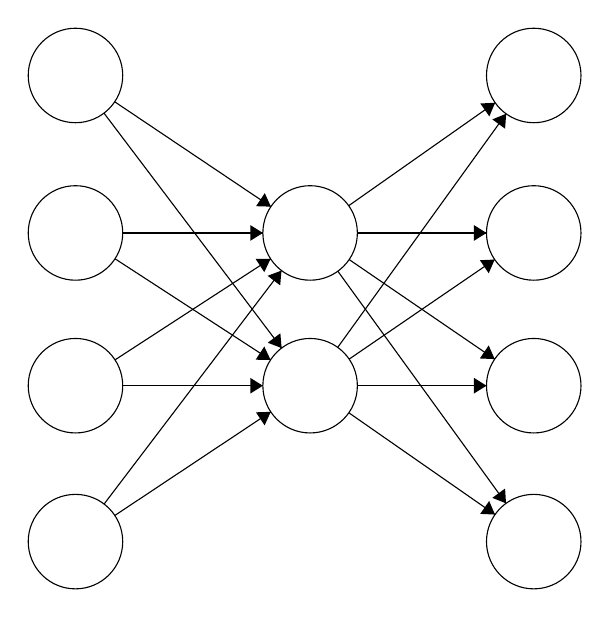
\begin{tikzpicture}[scale=0.2]
\tikzstyle{every node}+=[inner sep=0pt]
\draw [black] (21.5,-13.4) circle (3);
\draw [black] (21.5,-23.4) circle (3);
\draw [black] (21.5,-33.1) circle (3);
\draw [black] (36.4,-23.4) circle (3);
\draw [black] (36.4,-33.1) circle (3);
\draw [black] (50.6,-23.4) circle (3);
\draw [black] (21.5,-43) circle (3);
\draw [black] (50.6,-33.1) circle (3);
\draw [black] (50.6,-43) circle (3);
\draw [black] (50.6,-13.4) circle (3);
\draw [black] (24.5,-33.1) -- (33.4,-33.1);
\fill [black] (33.4,-33.1) -- (32.6,-32.6) -- (32.6,-33.6);
\draw [black] (24.01,-31.46) -- (33.89,-25.04);
\fill [black] (33.89,-25.04) -- (32.94,-25.05) -- (33.49,-25.89);
\draw [black] (24.5,-23.4) -- (33.4,-23.4);
\fill [black] (33.4,-23.4) -- (32.6,-22.9) -- (32.6,-23.9);
\draw [black] (24.01,-25.04) -- (33.89,-31.46);
\fill [black] (33.89,-31.46) -- (33.49,-30.61) -- (32.94,-31.45);
\draw [black] (23.99,-15.07) -- (33.91,-21.73);
\fill [black] (33.91,-21.73) -- (33.52,-20.87) -- (32.97,-21.7);
\draw [black] (23.31,-15.79) -- (34.59,-30.71);
\fill [black] (34.59,-30.71) -- (34.51,-29.77) -- (33.71,-30.37);
\draw [black] (39.4,-23.4) -- (47.6,-23.4);
\fill [black] (47.6,-23.4) -- (46.8,-22.9) -- (46.8,-23.9);
\draw [black] (38.88,-31.41) -- (48.12,-25.09);
\fill [black] (48.12,-25.09) -- (47.18,-25.13) -- (47.74,-25.96);
\draw [black] (24,-41.34) -- (33.9,-34.76);
\fill [black] (33.9,-34.76) -- (32.96,-34.79) -- (33.51,-35.62);
\draw [black] (23.32,-40.61) -- (34.58,-25.79);
\fill [black] (34.58,-25.79) -- (33.7,-26.12) -- (34.5,-26.73);
\draw [black] (38.85,-21.67) -- (48.15,-15.13);
\fill [black] (48.15,-15.13) -- (47.21,-15.18) -- (47.78,-16);
\draw [black] (38.88,-25.09) -- (48.12,-31.41);
\fill [black] (48.12,-31.41) -- (47.74,-30.54) -- (47.18,-31.37);
\draw [black] (38.16,-25.83) -- (48.84,-40.57);
\fill [black] (48.84,-40.57) -- (48.78,-39.63) -- (47.97,-40.22);
\draw [black] (38.15,-30.67) -- (48.85,-15.83);
\fill [black] (48.85,-15.83) -- (47.97,-16.19) -- (48.78,-16.78);
\draw [black] (39.4,-33.1) -- (47.6,-33.1);
\fill [black] (47.6,-33.1) -- (46.8,-32.6) -- (46.8,-33.6);
\draw [black] (38.86,-34.82) -- (48.14,-41.28);
\fill [black] (48.14,-41.28) -- (47.77,-40.42) -- (47.2,-41.24);
\end{tikzpicture}
\caption{\label{fig:autoencoder}Autoencoder de tres capas. Tiene 4 variables de entrada y genera una codificación en 2 variables} 
\end{figure}

El interés de los autoencoders reside en restringirlos, mediante la estructura de la red u otros parámetros, de forma que sean incapaces de simplemente aprender la función identidad. Así, la codificación que aprenden contiene información útil acerca de los datos de entrada, ya que se le fuerza a descartar los aspectos que no sean representativos. Si la codificación, además, es de menor dimensionalidad que la entrada, se puede utilizar el autoencoder como reductor de la dimensionalidad.

El concepto de los autoencoders no es nuevo, pero hasta hace unos años no se habían desarrollado técnicas para un entrenamiento eficiente. La aparición de SGD y sus derivados (\autoref{sec:dl-opt}) permitieron entrenar redes profundas de forma rápida, en particular los autoencoders. Además, \textcite{hinton2006autoencoder} introdujeron una técnica de entrenamiento basada en un cálculo de pesos iniciales previo y un posterior ajuste.

Existen diferentes variantes de los autoencoders según su estructura y función de coste, a continuación estudiamos las principales.

\subsubsection{Autoencoders infracompletos}

La primera restricción sencilla que permite obtener información interesante a partir del entrenamiento de un autoencoder es reducir la dimensión de la capa interna respecto de la de entrada, como se ve en el ejemplo de la \autoref{fig:autoencoder}. La representación de los datos que aprende este autoencoder se puede denominar \textit{infracompleta} (del inglés \textit{undercomplete}). Al entrenar un autoencoder de este tipo, los aspectos más representativos de los datos se quedan en la codificación porque sirven para reconstruirlos.

El proceso de aprendizaje consiste en minimizar una función de coste del tipo
\[
  L(x,g(f(x)))~,
\]
donde $L$ da una medida de la diferencia entre la entrada y su reconstrucción, como puede ser el error cuadrático medio.

Adicionalmente, se puede añadir un término de \textit{regularización} $\Omega$ junto a la función $L$, que dependa de los valores de la capa de codificación y añada ciertas propiedades deseadas al autoencoder. Algunas de las variaciones que se mencionan a continuación surgen a partir de esta generalización.

\subsubsection{Autoencoders dispersos}

Un autoencoder disperso (\textit{sparse autoencoder)} es simplemente un autoencoder cuya función de coste involucra, además del error cometido en la reconstrucción, una penalización de dispersión sobre la codificación $h$:
\[
  L(x,g(f(x)))+\Omega(h)~.
\]

La penalización de dispersión fuerza al autoencoder a aprender representaciones (infracompletas o sobrecompletas) en las que muy pocas unidades están activas, es decir, la mayor parte dan salida nula. Por esto, los autoencoders dispersos son muy útiles para la construcción de características que se pueden usar en una tarea de clasificación.

\subsubsection{Autoencoders con eliminación de ruido}

Otra tarea que puede aprender un autoencoder es la reparación del ruido en instancias (\textit{denoising autoencoder)}. Para ello, si tenemos para cada instancia $x$ una copia $\tilde x$ a la que se le ha introducido algún tipo de ruido, entrenamos un autoencoder que minimice la función
\[
  L(x, g(f(\tilde x)))~.
\]

De esta forma, el autoencoder se ve forzado a aprender la distribución de los datos de forma implícita, y se hace robusto al ruido. Una vez entrenado, podremos inyectar nuevas instancias ruidosas en la red y recuperar instancias limpias en la capa de salida.

\subsubsection{Autoencoders contractivos}

Un autoencoder contractivo (\textit{contractive autoencoder}) es un autoencoder con una regularización del tipo
\[
  \Omega(h)=\lambda\norm{\frac{\partial f(x)}{\partial x}}^2_F~,
\]
que hace que las parciales de f tiendan a ser lo más pequeñas posible.

Los autoencoders contractivos son robustos a perturbaciones locales en los datos de entrada, es decir, si una instancia $x$ se aplica en $f(x)$, entonces una instancia vecina $x'$ muy cercana a $x$ se aplicará también cerca de $f(x)$. Sin embargo, si los puntos $x$ y $x'$ son lejanos, sus imágenes por $f$ pueden ser aún más lejanas, de ahí la naturaleza local del comportamiento del autoencoder. Intuitivamente, se puede considerar que el autoencoder ``contrae'' el vecindario de cada instancia.

Una aplicación de los autoencoders contractivos es realizar aprendizaje de variedades (\textit{manifold learning}) sobre los datos.

%\subsubsection{Autoencoders variacionales}

\subsection{Entrenamiento de
  autoencoders}\label{entrenamiento-de-autoencoders}

Para el entrenamiento de autoencoders, es posible utilizar las técnicas que se han estudiado anteriormente, en concreto la propagación hacia atrás (\autoref{sec:backprop}) para calcular gradientes y los algoritmos basados en gradiente descendente estocástico (\autoref{sec:dl-opt}) para optimizar la función objetivo.

Sin embargo, al emplear autoencoders muy profundos este aprendizaje se puede tornar un proceso muy lento, por el hecho de que la inicialización de pesos no utiliza información acerca de los datos. Para solventar este problema se puede añadir una fase previa de pre-entrenamiento que encuentra unos pesos que acercan el autoencoder a un mínimo local, tras lo cual la fase de aprendizaje se emplea para realizar ajustes sobre dichos pesos \autocite{hinton2006autoencoder}. Este mismo proceso de entrenamiento es el que se utiliza en las \textit{Deep Belief Network}, que después se pueden entrenar adicionalmente para tareas supervisadas \autocite{hinton2006dbn}.

\subsubsection{Pre-entrenamiento}\label{pre-entrenamiento}

En esta fase, se toman parejas de capas consecutivas de la capa codificadora del autoencoder, comenzando por la de entrada y la siguiente, y se entrenan RBMs para cada una.

\begin{figure}[hbtp]
  \centering
  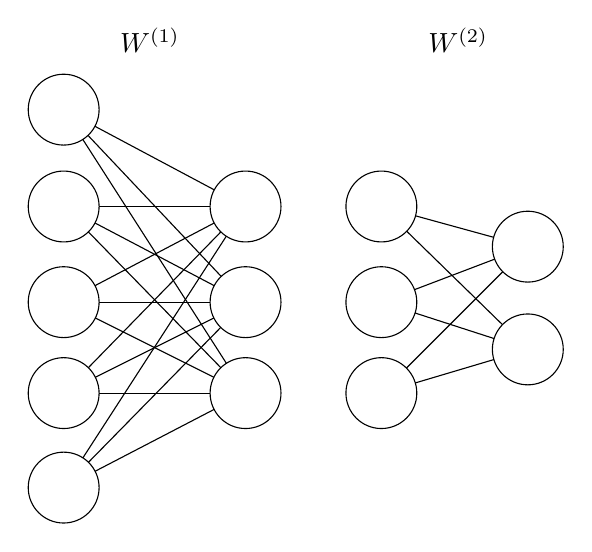
\begin{tikzpicture}[scale=0.15]
\tikzstyle{every node}+=[inner sep=0pt]
\draw [black] (13.9,-15.6) circle (3);
\draw [black] (13.9,-23.8) circle (3);
\draw [black] (13.9,-31.9) circle (3);
\draw [black] (13.9,-39.6) circle (3);
\draw [black] (13.9,-47.6) circle (3);
\draw [black] (29.3,-23.8) circle (3);
\draw [black] (29.3,-31.9) circle (3);
\draw [black] (29.3,-39.6) circle (3);
\draw [black] (40.8,-23.8) circle (3);
\draw [black] (40.8,-31.9) circle (3);
\draw [black] (40.8,-39.6) circle (3);
\draw [black] (53.2,-27.2) circle (3);
\draw [black] (53.2,-35.9) circle (3);
\draw (21.2,-9.7) node {$W^{(1)}$};
\draw (47.3,-9.7) node {$W^{(2)}$};
\draw [black] (16.55,-17.01) -- (26.65,-22.39);
%\fill [black] (26.65,-22.39) -- (26.18,-21.57) -- (25.71,-22.46);
\draw [black] (15.96,-17.78) -- (27.24,-29.72);
%\fill [black] (27.24,-29.72) -- (27.05,-28.79) -- (26.33,-29.48);
\draw [black] (15.52,-18.12) -- (27.68,-37.08);
%fill [black] (27.68,-37.08) -- (27.67,-36.13) -- (26.83,-36.67);
\draw [black] (16.9,-23.8) -- (26.3,-23.8);
%\fill [black] (26.3,-23.8) -- (25.5,-23.3) -- (25.5,-24.3);
\draw [black] (16.56,-25.2) -- (26.64,-30.5);
%\fill [black] (26.64,-30.5) -- (26.17,-29.69) -- (25.7,-30.57);
\draw [black] (15.99,-25.95) -- (27.21,-37.45);
%\fill [black] (27.21,-37.45) -- (27.01,-36.53) -- (26.29,-37.23);
\draw [black] (16.56,-30.5) -- (26.64,-25.2);
%\fill [black] (26.64,-25.2) -- (25.7,-25.13) -- (26.17,-26.01);
\draw [black] (16.9,-31.9) -- (26.3,-31.9);
%\fill [black] (26.3,-31.9) -- (25.5,-31.4) -- (25.5,-32.4);
\draw [black] (16.58,-33.24) -- (26.62,-38.26);
%\fill [black] (26.62,-38.26) -- (26.12,-37.45) -- (25.68,-38.35);
\draw [black] (15.99,-37.45) -- (27.21,-25.95);
%\fill [black] (27.21,-25.95) -- (26.29,-26.17) -- (27.01,-26.87);
\draw [black] (16.58,-38.26) -- (26.62,-33.24);
%\fill [black] (26.62,-33.24) -- (25.68,-33.15) -- (26.12,-34.05);
\draw [black] (16.9,-39.6) -- (26.3,-39.6);
%\fill [black] (26.3,-39.6) -- (25.5,-39.1) -- (25.5,-40.1);
\draw [black] (15.53,-45.08) -- (27.67,-26.32);
%\fill [black] (27.67,-26.32) -- (26.82,-26.72) -- (27.66,-27.26);
\draw [black] (16,-45.46) -- (27.2,-34.04);
%\fill [black] (27.2,-34.04) -- (26.28,-34.26) -- (27,-34.96);
\draw [black] (16.56,-46.22) -- (26.64,-40.98);
%\fill [black] (26.64,-40.98) -- (25.7,-40.91) -- (26.16,-41.8);
\draw [black] (43.69,-24.59) -- (50.31,-26.41);
%\fill [black] (50.31,-26.41) -- (49.67,-25.71) -- (49.4,-26.68);
\draw [black] (43.61,-30.84) -- (50.39,-28.26);
%\fill [black] (50.39,-28.26) -- (49.47,-28.08) -- (49.82,-29.01);
\draw [black] (42.92,-37.48) -- (51.08,-29.32);
%\fill [black] (51.08,-29.32) -- (50.16,-29.53) -- (50.87,-30.24);
\draw [black] (42.95,-25.9) -- (51.05,-33.8);
%\fill [black] (51.05,-33.8) -- (50.83,-32.89) -- (50.13,-33.6);
\draw [black] (43.66,-32.82) -- (50.34,-34.98);
%\fill [black] (50.34,-34.98) -- (49.74,-34.26) -- (49.43,-35.21);
\draw [black] (43.67,-38.74) -- (50.33,-36.76);
\end{tikzpicture}
  \caption[Pre-entrenamiento de un autoencoder]{Pre-entrenamiento de un autoencoder de 5 capas, con un codificador de 5, 3 y 2 neuronas en la primera, segunda y tercera capa respectivamente}
  \label{fig:ae-pretrain}
\end{figure}

En el ejemplo de la \autoref{fig:ae-pretrain}, se toma la primera capa y la segunda y se entrena una RBM con los datos de entrada. A continuación, la segunda y la tercera forman otra RBM que se entrena con los datos resultantes de atravesar la primera RBM con los datos de entrada. De esta forma, se obtienen sendas matrices de pesos $W^{(1)}$ y $W^{(2)}$.

\subsubsection{Ajuste fino}\label{ajuste-fino}

Una vez obtenidos unos pesos iniciales mediante el pre-entrenamiento, se ``desenrolla'' la estructura completa del autoencoder, manteniendo los pesos aprendidos tanto en el codificador como en el decodificador, como se puede observar en la \autoref{fig:ae-unroll}. Por último, se ejecuta un optimizador basado en SGD para ajustar estos pesos y los sesgos, para minimizar la función de coste requerida, según el tipo de autoencoder construido.

\begin{figure}[hbtp]
  \centering
  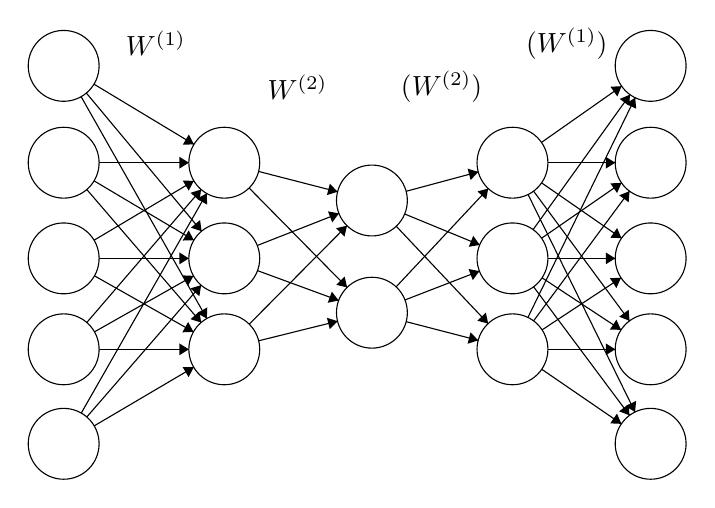
\begin{tikzpicture}[scale=0.15]
\tikzstyle{every node}+=[inner sep=0pt]
\draw [black] (15.7,-15.6) circle (3);
\draw [black] (15.7,-23.8) circle (3);
\draw [black] (15.7,-31.9) circle (3);
\draw [black] (15.7,-39.6) circle (3);
\draw [black] (15.7,-47.6) circle (3);
\draw [black] (29.3,-23.8) circle (3);
\draw [black] (29.3,-31.9) circle (3);
\draw [black] (29.3,-39.6) circle (3);
\draw [black] (41.8,-27) circle (3);
\draw [black] (41.8,-36.5) circle (3);
\draw (23.5,-13.7) node {$W^{(1)}$};
\draw (35.5,-17.4) node {$W^{(2)}$};
\draw [black] (53.7,-23.8) circle (3);
\draw [black] (53.7,-31.9) circle (3);
\draw [black] (53.7,-39.6) circle (3);
\draw [black] (65.4,-15.6) circle (3);
\draw [black] (65.4,-23.8) circle (3);
\draw [black] (65.4,-31.9) circle (3);
\draw [black] (65.4,-39.6) circle (3);
\draw [black] (65.4,-47.6) circle (3);
\draw (47.7,-17.4) node {$\Tr{(W^{(2)})}$};
\draw (58.3,-13.7) node {$\Tr{(W^{(1)})}$};
\draw [black] (18.27,-17.15) -- (26.73,-22.25);
\fill [black] (26.73,-22.25) -- (26.3,-21.41) -- (25.79,-22.27);
\draw [black] (17.62,-17.9) -- (27.38,-29.6);
\fill [black] (27.38,-29.6) -- (27.25,-28.66) -- (26.48,-29.3);
\draw [black] (17.18,-18.21) -- (27.82,-36.99);
\fill [black] (27.82,-36.99) -- (27.86,-36.05) -- (26.99,-36.54);
\draw [black] (18.7,-23.8) -- (26.3,-23.8);
\fill [black] (26.3,-23.8) -- (25.5,-23.3) -- (25.5,-24.3);
\draw [black] (18.28,-25.34) -- (26.72,-30.36);
\fill [black] (26.72,-30.36) -- (26.29,-29.53) -- (25.78,-30.39);
\draw [black] (17.66,-26.07) -- (27.34,-37.33);
\fill [black] (27.34,-37.33) -- (27.2,-36.39) -- (26.44,-37.05);
\draw [black] (18.28,-30.36) -- (26.72,-25.34);
\fill [black] (26.72,-25.34) -- (25.78,-25.31) -- (26.29,-26.17);
\draw [black] (18.7,-31.9) -- (26.3,-31.9);
\fill [black] (26.3,-31.9) -- (25.5,-31.4) -- (25.5,-32.4);
\draw [black] (18.31,-33.38) -- (26.69,-38.12);
\fill [black] (26.69,-38.12) -- (26.24,-37.29) -- (25.75,-38.16);
\draw [black] (17.66,-37.33) -- (27.34,-26.07);
\fill [black] (27.34,-26.07) -- (26.44,-26.35) -- (27.2,-27.01);
\draw [black] (18.31,-38.12) -- (26.69,-33.38);
\fill [black] (26.69,-33.38) -- (25.75,-33.34) -- (26.24,-34.21);
\draw [black] (18.7,-39.6) -- (26.3,-39.6);
\fill [black] (26.3,-39.6) -- (25.5,-39.1) -- (25.5,-40.1);
\draw [black] (17.19,-45) -- (27.81,-26.4);
\fill [black] (27.81,-26.4) -- (26.98,-26.85) -- (27.85,-27.35);
\draw [black] (17.66,-45.33) -- (27.34,-34.17);
\fill [black] (27.34,-34.17) -- (26.43,-34.44) -- (27.19,-35.1);
\draw [black] (18.29,-46.08) -- (26.71,-41.12);
\fill [black] (26.71,-41.12) -- (25.77,-41.1) -- (26.28,-41.96);
\draw [black] (32.21,-24.54) -- (38.89,-26.26);
\fill [black] (38.89,-26.26) -- (38.24,-25.57) -- (37.99,-26.54);
\draw [black] (32.09,-30.81) -- (39.01,-28.09);
\fill [black] (39.01,-28.09) -- (38.08,-27.92) -- (38.44,-28.85);
\draw [black] (31.41,-37.47) -- (39.69,-29.13);
\fill [black] (39.69,-29.13) -- (38.77,-29.35) -- (39.48,-30.05);
\draw [black] (31.4,-25.94) -- (39.7,-34.36);
\fill [black] (39.7,-34.36) -- (39.49,-33.44) -- (38.78,-34.14);
\draw [black] (32.12,-32.94) -- (38.98,-35.46);
\fill [black] (38.98,-35.46) -- (38.41,-34.72) -- (38.06,-35.66);
\draw [black] (32.21,-38.88) -- (38.89,-37.22);
\fill [black] (38.89,-37.22) -- (37.99,-36.93) -- (38.23,-37.9);
\draw [black] (44.7,-37.26) -- (50.8,-38.84);
\fill [black] (50.8,-38.84) -- (50.15,-38.16) -- (49.9,-39.13);
\draw [black] (44.6,-35.42) -- (50.9,-32.98);
\fill [black] (50.9,-32.98) -- (49.98,-32.8) -- (50.34,-33.74);
\draw [black] (43.85,-34.31) -- (51.65,-25.99);
\fill [black] (51.65,-25.99) -- (50.74,-26.23) -- (51.47,-26.91);
\draw [black] (44.7,-26.22) -- (50.8,-24.58);
\fill [black] (50.8,-24.58) -- (49.9,-24.3) -- (50.16,-25.27);
\draw [black] (44.57,-28.14) -- (50.93,-30.76);
\fill [black] (50.93,-30.76) -- (50.38,-29.99) -- (50,-30.92);
\draw [black] (43.86,-29.18) -- (51.64,-37.42);
\fill [black] (51.64,-37.42) -- (51.45,-36.49) -- (50.73,-37.18);
\draw [black] (56.16,-22.08) -- (62.94,-17.32);
\fill [black] (62.94,-17.32) -- (62,-17.37) -- (62.58,-18.19);
\draw [black] (56.7,-23.8) -- (62.4,-23.8);
\fill [black] (62.4,-23.8) -- (61.6,-23.3) -- (61.6,-24.3);
\draw [black] (56.17,-25.51) -- (62.93,-30.19);
\fill [black] (62.93,-30.19) -- (62.56,-29.33) -- (61.99,-30.15);
\draw [black] (56.21,-33.55) -- (62.89,-37.95);
\fill [black] (62.89,-37.95) -- (62.5,-37.09) -- (61.95,-37.93);
\draw [black] (55.49,-26.21) -- (63.61,-37.19);
\fill [black] (63.61,-37.19) -- (63.54,-36.25) -- (62.74,-36.84);
\draw [black] (55.02,-26.49) -- (64.08,-44.91);
\fill [black] (64.08,-44.91) -- (64.17,-43.97) -- (63.27,-44.41);
\draw [black] (55.45,-29.46) -- (63.65,-18.04);
\fill [black] (63.65,-18.04) -- (62.78,-18.4) -- (63.59,-18.98);
\draw [black] (56.17,-30.19) -- (62.93,-25.51);
\fill [black] (62.93,-25.51) -- (61.99,-25.55) -- (62.56,-26.37);
\draw [black] (56.7,-31.9) -- (62.4,-31.9);
\fill [black] (62.4,-31.9) -- (61.6,-31.4) -- (61.6,-32.4);
\draw [black] (55.49,-34.31) -- (63.61,-45.19);
\fill [black] (63.61,-45.19) -- (63.53,-44.25) -- (62.73,-44.85);
\draw [black] (55.01,-36.9) -- (64.09,-18.3);
\fill [black] (64.09,-18.3) -- (63.29,-18.8) -- (64.18,-19.23);
\draw [black] (55.49,-37.19) -- (63.61,-26.21);
\fill [black] (63.61,-26.21) -- (62.74,-26.56) -- (63.54,-27.15);
\draw [black] (56.21,-37.95) -- (62.89,-33.55);
\fill [black] (62.89,-33.55) -- (61.95,-33.57) -- (62.5,-34.41);
\draw [black] (56.7,-39.6) -- (62.4,-39.6);
\fill [black] (62.4,-39.6) -- (61.6,-39.1) -- (61.6,-40.1);
\draw [black] (56.18,-41.29) -- (62.92,-45.91);
\fill [black] (62.92,-45.91) -- (62.55,-45.04) -- (61.98,-45.87);
\end{tikzpicture}
  \caption[Desenrollado del autoencoder]{Desenrollado del autoencoder, manteniendo las matrices de pesos aprendidas en el pre-entrenamiento}
  \label{fig:ae-unroll}
\end{figure}

Durante la optimización, los datos se hacen pasar por la red (propagación hacia adelante) en minilotes, es decir, cada gradiente no se calcula respecto del conjunto completo de instancias sino de una muestra de ellas de un tamaño fijo dado. De esta forma, cada iteración del algoritmo es más rápida, sin perder capacidad de generalización ya que en cada iteración hay oportunidad de escoger nuevas instancias. El número de iteraciones también se conoce como número de \emph{épocas}, y suele ser un parámetro escogido por el usuario. Según la rapidez de la convergencia del algoritmo, serán necesarias más o menos épocas para llegar a un mínimo local.